\documentclass[1p]{elsarticle_modified}
%\bibliographystyle{elsarticle-num}

%\usepackage[colorlinks]{hyperref}
%\usepackage{abbrmath_seonhwa} %\Abb, \Ascr, \Acal ,\Abf, \Afrak
\usepackage{amsfonts}
\usepackage{amssymb}
\usepackage{amsmath}
\usepackage{amsthm}
\usepackage{scalefnt}
\usepackage{amsbsy}
\usepackage{kotex}
\usepackage{caption}
\usepackage{subfig}
\usepackage{color}
\usepackage{graphicx}
\usepackage{xcolor} %% white, black, red, green, blue, cyan, magenta, yellow
\usepackage{float}
\usepackage{setspace}
\usepackage{hyperref}

\usepackage{tikz}
\usetikzlibrary{arrows}

\usepackage{multirow}
\usepackage{array} % fixed length table
\usepackage{hhline}

%%%%%%%%%%%%%%%%%%%%%
\makeatletter
\renewcommand*\env@matrix[1][\arraystretch]{%
	\edef\arraystretch{#1}%
	\hskip -\arraycolsep
	\let\@ifnextchar\new@ifnextchar
	\array{*\c@MaxMatrixCols c}}
\makeatother %https://tex.stackexchange.com/questions/14071/how-can-i-increase-the-line-spacing-in-a-matrix
%%%%%%%%%%%%%%%

\usepackage[normalem]{ulem}

\newcommand{\msout}[1]{\ifmmode\text{\sout{\ensuremath{#1}}}\else\sout{#1}\fi}
%SOURCE: \msout is \stkout macro in https://tex.stackexchange.com/questions/20609/strikeout-in-math-mode

\newcommand{\cancel}[1]{
	\ifmmode
	{\color{red}\msout{#1}}
	\else
	{\color{red}\sout{#1}}
	\fi
}

\newcommand{\add}[1]{
	{\color{blue}\uwave{#1}}
}

\newcommand{\replace}[2]{
	\ifmmode
	{\color{red}\msout{#1}}{\color{blue}\uwave{#2}}
	\else
	{\color{red}\sout{#1}}{\color{blue}\uwave{#2}}
	\fi
}

\newcommand{\Sol}{\mathcal{S}} %segment
\newcommand{\D}{D} %diagram
\newcommand{\A}{\mathcal{A}} %arc


%%%%%%%%%%%%%%%%%%%%%%%%%%%%%5 test

\def\sl{\operatorname{\textup{SL}}(2,\Cbb)}
\def\psl{\operatorname{\textup{PSL}}(2,\Cbb)}
\def\quan{\mkern 1mu \triangleright \mkern 1mu}

\theoremstyle{definition}
\newtheorem{thm}{Theorem}[section]
\newtheorem{prop}[thm]{Proposition}
\newtheorem{lem}[thm]{Lemma}
\newtheorem{ques}[thm]{Question}
\newtheorem{cor}[thm]{Corollary}
\newtheorem{defn}[thm]{Definition}
\newtheorem{exam}[thm]{Example}
\newtheorem{rmk}[thm]{Remark}
\newtheorem{alg}[thm]{Algorithm}

\newcommand{\I}{\sqrt{-1}}
\begin{document}

%\begin{frontmatter}
%
%\title{Boundary parabolic representations of knots up to 8 crossings}
%
%%% Group authors per affiliation:
%\author{Yunhi Cho} 
%\address{Department of Mathematics, University of Seoul, Seoul, Korea}
%\ead{yhcho@uos.ac.kr}
%
%
%\author{Seonhwa Kim} %\fnref{s_kim}}
%\address{Center for Geometry and Physics, Institute for Basic Science, Pohang, 37673, Korea}
%\ead{ryeona17@ibs.re.kr}
%
%\author{Hyuk Kim}
%\address{Department of Mathematical Sciences, Seoul National University, Seoul 08826, Korea}
%\ead{hyukkim@snu.ac.kr}
%
%\author{Seokbeom Yoon}
%\address{Department of Mathematical Sciences, Seoul National University, Seoul, 08826,  Korea}
%\ead{sbyoon15@snu.ac.kr}
%
%\begin{abstract}
%We find all boundary parabolic representation of knots up to 8 crossings.
%
%\end{abstract}
%\begin{keyword}
%    \MSC[2010] 57M25 
%\end{keyword}
%
%\end{frontmatter}

%\linenumbers
%\tableofcontents
%
\newcommand\colored[1]{\textcolor{white}{\rule[-0.35ex]{0.8em}{1.4ex}}\kern-0.8em\color{red} #1}%
%\newcommand\colored[1]{\textcolor{white}{ #1}\kern-2.17ex	\textcolor{white}{ #1}\kern-1.81ex	\textcolor{white}{ #1}\kern-2.15ex\color{red}#1	}

{\Large $\underline{10_{45}~(K10a_{25})}$}

\setlength{\tabcolsep}{10pt}
\renewcommand{\arraystretch}{1.6}
\vspace{1cm}\begin{tabular}{m{100pt}>{\centering\arraybackslash}m{274pt}}
\multirow{5}{120pt}{
	\centering
	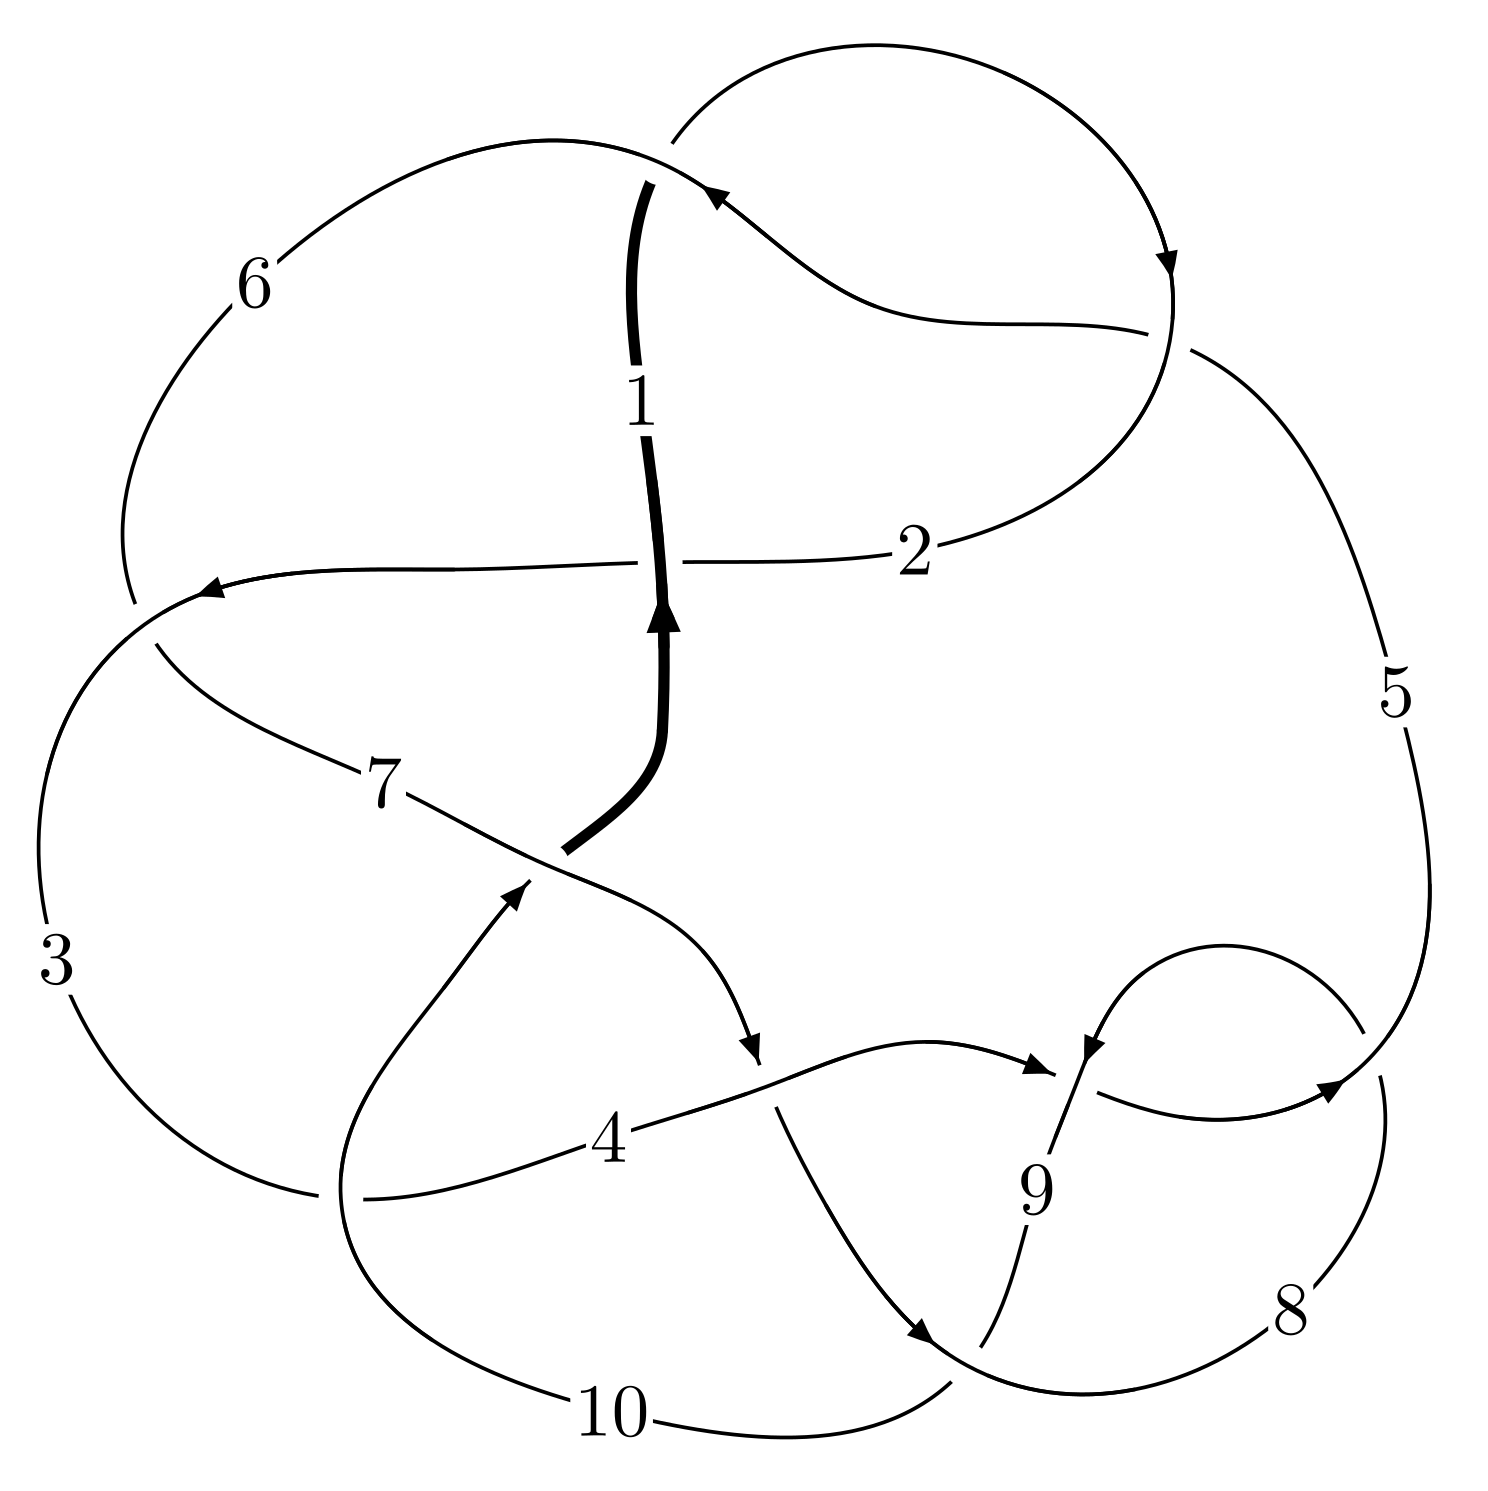
\includegraphics[width=112pt]{../../../GIT/diagram.site/Diagrams/png/129_10_45.png}\\
\ \ \ A knot diagram\footnotemark}&
\allowdisplaybreaks
\textbf{Linearized knot diagam} \\
\cline{2-2}
 &
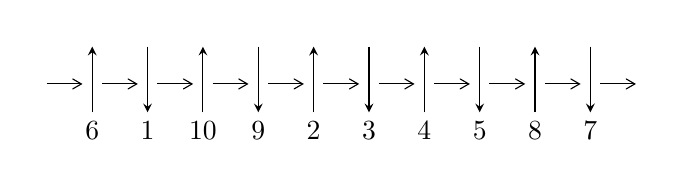
\begin{tikzpicture}[x=20pt, y=17pt]
	% nodes
	\node (C0) at (0, 0) {};
	\node (C1) at (1, 0) {};
	\node (C1U) at (1, +1) {};
	\node (C1D) at (1, -1) {6};

	\node (C2) at (2, 0) {};
	\node (C2U) at (2, +1) {};
	\node (C2D) at (2, -1) {1};

	\node (C3) at (3, 0) {};
	\node (C3U) at (3, +1) {};
	\node (C3D) at (3, -1) {10};

	\node (C4) at (4, 0) {};
	\node (C4U) at (4, +1) {};
	\node (C4D) at (4, -1) {9};

	\node (C5) at (5, 0) {};
	\node (C5U) at (5, +1) {};
	\node (C5D) at (5, -1) {2};

	\node (C6) at (6, 0) {};
	\node (C6U) at (6, +1) {};
	\node (C6D) at (6, -1) {3};

	\node (C7) at (7, 0) {};
	\node (C7U) at (7, +1) {};
	\node (C7D) at (7, -1) {4};

	\node (C8) at (8, 0) {};
	\node (C8U) at (8, +1) {};
	\node (C8D) at (8, -1) {5};

	\node (C9) at (9, 0) {};
	\node (C9U) at (9, +1) {};
	\node (C9D) at (9, -1) {8};

	\node (C10) at (10, 0) {};
	\node (C10U) at (10, +1) {};
	\node (C10D) at (10, -1) {7};
	\node (C11) at (11, 0) {};

	% arrows
	\draw[->,>={angle 60}]
	(C0) edge (C1) (C1) edge (C2) (C2) edge (C3) (C3) edge (C4) (C4) edge (C5) (C5) edge (C6) (C6) edge (C7) (C7) edge (C8) (C8) edge (C9) (C9) edge (C10) (C10) edge (C11) ;	\draw[->,>=stealth]
	(C1D) edge (C1U) (C2U) edge (C2D) (C3D) edge (C3U) (C4U) edge (C4D) (C5D) edge (C5U) (C6U) edge (C6D) (C7D) edge (C7U) (C8U) edge (C8D) (C9D) edge (C9U) (C10U) edge (C10D) ;
	\end{tikzpicture} \\
\hhline{~~} \\& 
\textbf{Solving Sequence} \\ \cline{2-2} 
 &
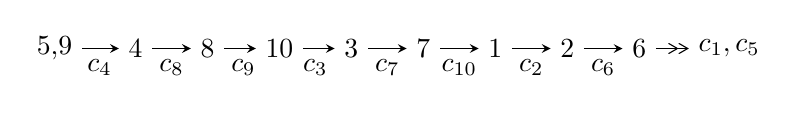
\begin{tikzpicture}[x=26pt, y=7pt]
	% node
	\node (A0) at (-1/8, 0) {5,9};
	\node (A1) at (1, 0) {4};
	\node (A2) at (2, 0) {8};
	\node (A3) at (3, 0) {10};
	\node (A4) at (4, 0) {3};
	\node (A5) at (5, 0) {7};
	\node (A6) at (6, 0) {1};
	\node (A7) at (7, 0) {2};
	\node (A8) at (8, 0) {6};
	\node (C1) at (1/2, -1) {$c_{4}$};
	\node (C2) at (3/2, -1) {$c_{8}$};
	\node (C3) at (5/2, -1) {$c_{9}$};
	\node (C4) at (7/2, -1) {$c_{3}$};
	\node (C5) at (9/2, -1) {$c_{7}$};
	\node (C6) at (11/2, -1) {$c_{10}$};
	\node (C7) at (13/2, -1) {$c_{2}$};
	\node (C8) at (15/2, -1) {$c_{6}$};
	\node (A9) at (37/4, 0) {$c_{1},c_{5}$};

	% edge
	\draw[->,>=stealth]	
	(A0) edge (A1) (A1) edge (A2) (A2) edge (A3) (A3) edge (A4) (A4) edge (A5) (A5) edge (A6) (A6) edge (A7) (A7) edge (A8) ;
	\draw[->>,>={angle 60}]	
	(A8) edge (A9);
\end{tikzpicture} \\ 

\end{tabular} \\

\footnotetext{
The image of knot diagram is generated by the software ``\textbf{Draw programme}" developed by Andrew Bartholomew(\url{http://www.layer8.co.uk/maths/draw/index.htm\#Running-draw}), where we modified some parts for our purpose(\url{https://github.com/CATsTAILs/LinksPainter}).
}\phantom \\ \newline 
\centering \textbf{Ideals for irreducible components\footnotemark of $X_{\text{par}}$} 
 
\begin{align*}
I^u_{1}&=\langle 
u^{44}- u^{43}+\cdots-2 u+1\rangle \\
\\
\end{align*}
\raggedright * 1 irreducible components of $\dim_{\mathbb{C}}=0$, with total 44 representations.\\
\footnotetext{All coefficients of polynomials are rational numbers. But the coefficients are sometimes approximated in decimal forms when there is not enough margin.}
\newpage
\renewcommand{\arraystretch}{1}
\centering \section*{I. $I^u_{1}= \langle u^{44}- u^{43}+\cdots-2 u+1 \rangle$}
\flushleft \textbf{(i) Arc colorings}\\
\begin{tabular}{m{7pt} m{180pt} m{7pt} m{180pt} }
\flushright $a_{5}=$&$\begin{pmatrix}1\\0\end{pmatrix}$ \\
\flushright $a_{9}=$&$\begin{pmatrix}0\\u\end{pmatrix}$ \\
\flushright $a_{4}=$&$\begin{pmatrix}1\\- u^2\end{pmatrix}$ \\
\flushright $a_{8}=$&$\begin{pmatrix}u\\u\end{pmatrix}$ \\
\flushright $a_{10}=$&$\begin{pmatrix}u^3\\u^3+u\end{pmatrix}$ \\
\flushright $a_{3}=$&$\begin{pmatrix}u^8+u^6+u^4+1\\u^8+2 u^6+2 u^4\end{pmatrix}$ \\
\flushright $a_{7}=$&$\begin{pmatrix}- u^3\\u^5+u^3+u\end{pmatrix}$ \\
\flushright $a_{1}=$&$\begin{pmatrix}- u^{11}-2 u^9-2 u^7+u^3\\u^{13}+3 u^{11}+5 u^9+4 u^7+2 u^5+u^3+u\end{pmatrix}$ \\
\flushright $a_{2}=$&$\begin{pmatrix}u^{32}+7 u^{30}+\cdots+2 u^{12}+1\\- u^{34}-8 u^{32}+\cdots-4 u^6- u^2\end{pmatrix}$ \\
\flushright $a_{6}=$&$\begin{pmatrix}u^{21}+4 u^{19}+9 u^{17}+12 u^{15}+12 u^{13}+10 u^{11}+9 u^9+6 u^7+3 u^5+u\\u^{21}+5 u^{19}+13 u^{17}+20 u^{15}+20 u^{13}+13 u^{11}+7 u^9+4 u^7+3 u^5+u^3+u\end{pmatrix}$\\&\end{tabular}
\flushleft \textbf{(ii) Obstruction class $= -1$}\\~\\
\flushleft \textbf{(iii) Cusp Shapes $= 4 u^{43}-4 u^{42}+\cdots+12 u-6$}\\~\\
\newpage\renewcommand{\arraystretch}{1}
\flushleft \textbf{(iv) u-Polynomials at the component}\newline \\
\begin{tabular}{m{50pt}|m{274pt}}
Crossings & \hspace{64pt}u-Polynomials at each crossing \\
\hline $$\begin{aligned}c_{1},c_{5}\end{aligned}$$&$\begin{aligned}
&u^{44}- u^{43}+\cdots-2 u+1
\end{aligned}$\\
\hline $$\begin{aligned}c_{2}\end{aligned}$$&$\begin{aligned}
&u^{44}+21 u^{43}+\cdots+2 u+1
\end{aligned}$\\
\hline $$\begin{aligned}c_{3}\end{aligned}$$&$\begin{aligned}
&u^{44}+5 u^{43}+\cdots+82 u+13
\end{aligned}$\\
\hline $$\begin{aligned}c_{4},c_{8}\end{aligned}$$&$\begin{aligned}
&u^{44}+u^{43}+\cdots+2 u+1
\end{aligned}$\\
\hline $$\begin{aligned}c_{6}\end{aligned}$$&$\begin{aligned}
&u^{44}+u^{43}+\cdots+68 u+17
\end{aligned}$\\
\hline $$\begin{aligned}c_{7}\end{aligned}$$&$\begin{aligned}
&u^{44}- u^{43}+\cdots-68 u+17
\end{aligned}$\\
\hline $$\begin{aligned}c_{9}\end{aligned}$$&$\begin{aligned}
&u^{44}-21 u^{43}+\cdots-2 u+1
\end{aligned}$\\
\hline $$\begin{aligned}c_{10}\end{aligned}$$&$\begin{aligned}
&u^{44}-5 u^{43}+\cdots-82 u+13
\end{aligned}$\\
\hline
\end{tabular}\\~\\
\newpage\renewcommand{\arraystretch}{1}
\flushleft \textbf{(v) Riley Polynomials at the component}\newline \\
\begin{tabular}{m{50pt}|m{274pt}}
Crossings & \hspace{64pt}Riley Polynomials at each crossing \\
\hline $$\begin{aligned}c_{1},c_{4},c_{5}\\c_{8}\end{aligned}$$&$\begin{aligned}
&y^{44}+21 y^{43}+\cdots+2 y+1
\end{aligned}$\\
\hline $$\begin{aligned}c_{2},c_{9}\end{aligned}$$&$\begin{aligned}
&y^{44}+5 y^{43}+\cdots+6 y+1
\end{aligned}$\\
\hline $$\begin{aligned}c_{3},c_{10}\end{aligned}$$&$\begin{aligned}
&y^{44}+9 y^{43}+\cdots+5314 y+169
\end{aligned}$\\
\hline $$\begin{aligned}c_{6},c_{7}\end{aligned}$$&$\begin{aligned}
&y^{44}-11 y^{43}+\cdots-4794 y+289
\end{aligned}$\\
\hline
\end{tabular}\\~\\
\newpage\flushleft \textbf{(vi) Complex Volumes and Cusp Shapes}
$$\begin{array}{c|c|c}  
\text{Solutions to }I^u_{1}& \I (\text{vol} + \sqrt{-1}CS) & \text{Cusp shape}\\
 \hline 
\begin{aligned}
u &= \phantom{-}0.219635 + 1.024160 I\end{aligned}
 & \phantom{-0.000000 } -1.08070 I & \phantom{-0.000000 -}     -6
0. 10   + 1.298529 I \\ \hline\begin{aligned}
u &= \phantom{-}0.219635 - 1.024160 I\end{aligned}
 & \phantom{-0.000000 -}1.08070 I & \phantom{-0.000000 }      -6
0. 10   - 1.298529 I \\ \hline\begin{aligned}
u &= -0.651337 + 0.622116 I\end{aligned}
 & -3.71248 + 6.51845 I & -4.95829 - 6.88419 I \\ \hline\begin{aligned}
u &= -0.651337 - 0.622116 I\end{aligned}
 & -3.71248 - 6.51845 I & -4.95829 + 6.88419 I \\ \hline\begin{aligned}
u &= -0.567171 + 0.946930 I\end{aligned}
 & -2.75664 - 1.75570 I & -3.52773 + 0.85914 I \\ \hline\begin{aligned}
u &= -0.567171 - 0.946930 I\end{aligned}
 & -2.75664 + 1.75570 I & -3.52773 - 0.85914 I \\ \hline\begin{aligned}
u &= \phantom{-}0.525013 + 0.980467 I\end{aligned}
 & -0.14884 - 2.53826 I & \phantom{-}0.24501 + 3.05915 I \\ \hline\begin{aligned}
u &= \phantom{-}0.525013 - 0.980467 I\end{aligned}
 & -0.14884 + 2.53826 I & \phantom{-}0.24501 - 3.05915 I \\ \hline\begin{aligned}
u &= -0.254705 + 1.115020 I\end{aligned}
 & \phantom{-}4.35508 - 1.04298 I & \phantom{-}6.65567 + 0.28795 I \\ \hline\begin{aligned}
u &= -0.254705 - 1.115020 I\end{aligned}
 & \phantom{-}4.35508 + 1.04298 I & \phantom{-}6.65567 - 0.28795 I \\ \hline\begin{aligned}
u &= -0.662694 + 0.538070 I\end{aligned}
 & -5.06451 - 1.08737 I & -7.53766 + 0.51091 I \\ \hline\begin{aligned}
u &= -0.662694 - 0.538070 I\end{aligned}
 & -5.06451 + 1.08737 I & -7.53766 - 0.51091 I \\ \hline\begin{aligned}
u &= \phantom{-}0.603028 + 0.598100 I\end{aligned}
 & -1.27162 - 1.94114 I & -1.79245 + 3.31415 I \\ \hline\begin{aligned}
u &= \phantom{-}0.603028 - 0.598100 I\end{aligned}
 & -1.27162 + 1.94114 I & -1.79245 - 3.31415 I \\ \hline\begin{aligned}
u &= \phantom{-}0.228645 + 1.128370 I\end{aligned}
 & \phantom{-}2.27286 + 5.97235 I & \phantom{-}3.25101 - 4.61402 I \\ \hline\begin{aligned}
u &= \phantom{-}0.228645 - 1.128370 I\end{aligned}
 & \phantom{-}2.27286 - 5.97235 I & \phantom{-}3.25101 + 4.61402 I \\ \hline\begin{aligned}
u &= -0.323792 + 1.114600 I\end{aligned}
 & \phantom{-}5.06451 + 1.08737 I & \phantom{-}7.53766 - 0.51091 I \\ \hline\begin{aligned}
u &= -0.323792 - 1.114600 I\end{aligned}
 & \phantom{-}5.06451 - 1.08737 I & \phantom{-}7.53766 + 0.51091 I \\ \hline\begin{aligned}
u &= -0.570170 + 1.011790 I\end{aligned}
 & -3.67003 + 5.88530 I & -4.74516 - 6.36553 I \\ \hline\begin{aligned}
u &= -0.570170 - 1.011790 I\end{aligned}
 & -3.67003 - 5.88530 I & -4.74516 + 6.36553 I \\ \hline\begin{aligned}
u &= \phantom{-}0.764138 + 0.339961 I\end{aligned}
 & -2.30812 + 8.68200 I & -3.24304 - 6.31705 I \\ \hline\begin{aligned}
u &= \phantom{-}0.764138 - 0.339961 I\end{aligned}
 & -2.30812 - 8.68200 I & -3.24304 + 6.31705 I \\ \hline\begin{aligned}
u &= \phantom{-}0.358424 + 1.122990 I\end{aligned}
 & \phantom{-}3.67003 - 5.88530 I & \phantom{-}4.74516 + 6.36553 I \\ \hline\begin{aligned}
u &= \phantom{-}0.358424 - 1.122990 I\end{aligned}
 & \phantom{-}3.67003 + 5.88530 I & \phantom{-}4.74516 - 6.36553 I \\ \hline\begin{aligned}
u &= \phantom{-}0.721497 + 0.387567 I\end{aligned}
 & -4.35508 + 1.04298 I & -6.65567 - 0.28795 I \\ \hline\begin{aligned}
u &= \phantom{-}0.721497 - 0.387567 I\end{aligned}
 & -4.35508 - 1.04298 I & -6.65567 + 0.28795 I \\ \hline\begin{aligned}
u &= -0.737315 + 0.329710 I\end{aligned}
 & \phantom{-0.000000 } -3.75579 I & \phantom{-0.000000 -}0. + 2.66459 I \\ \hline\begin{aligned}
u &= -0.737315 - 0.329710 I\end{aligned}
 & \phantom{-0.000000 -}3.75579 I & \phantom{-0.000000 } 0. - 2.66459 I \\ \hline\begin{aligned}
u &= \phantom{-}0.494931 + 1.113460 I\end{aligned}
 & \phantom{-}2.75664 - 1.75570 I & \phantom{-}3.52773 + 0.85914 I \\ \hline\begin{aligned}
u &= \phantom{-}0.494931 - 1.113460 I\end{aligned}
 & \phantom{-}2.75664 + 1.75570 I & \phantom{-}3.52773 - 0.85914 I\\
 \hline 
 \end{array}$$\newpage$$\begin{array}{c|c|c}  
\text{Solutions to }I^u_{1}& \I (\text{vol} + \sqrt{-1}CS) & \text{Cusp shape}\\
 \hline 
\begin{aligned}
u &= -0.523186 + 1.116830 I\end{aligned}
 & \phantom{-}3.71248 + 6.51845 I & \phantom{-}4.95829 - 6.88419 I \\ \hline\begin{aligned}
u &= -0.523186 - 1.116830 I\end{aligned}
 & \phantom{-}3.71248 - 6.51845 I & \phantom{-}4.95829 + 6.88419 I \\ \hline\begin{aligned}
u &= \phantom{-}0.568139 + 1.097600 I\end{aligned}
 & -2.27286 - 5.97235 I & -3.25101 + 4.61402 I \\ \hline\begin{aligned}
u &= \phantom{-}0.568139 - 1.097600 I\end{aligned}
 & -2.27286 + 5.97235 I & -3.25101 - 4.61402 I \\ \hline\begin{aligned}
u &= \phantom{-}0.326591 + 0.684448 I\end{aligned}
 & \phantom{-0.000000 } -1.50871 I & \phantom{-0.000000 -}0. + 4.89247 I \\ \hline\begin{aligned}
u &= \phantom{-}0.326591 - 0.684448 I\end{aligned}
 & \phantom{-0.000000 -}1.50871 I & \phantom{-0.000000 } 0. - 4.89247 I \\ \hline\begin{aligned}
u &= -0.560153 + 1.120390 I\end{aligned}
 & \phantom{-}2.30812 + 8.68200 I & \phantom{-}3.24304 - 6.31705 I \\ \hline\begin{aligned}
u &= -0.560153 - 1.120390 I\end{aligned}
 & \phantom{-}2.30812 - 8.68200 I & \phantom{-}3.24304 + 6.31705 I \\ \hline\begin{aligned}
u &= \phantom{-}0.570711 + 1.124900 I\end{aligned}
 & \phantom{-0.000000 } -13.7161 I & \phantom{-0.000000 -}0. + 10.01278 I \\ \hline\begin{aligned}
u &= \phantom{-}0.570711 - 1.124900 I\end{aligned}
 & \phantom{-0.000000 -}13.7161 I & \phantom{-0.000000 } 0. - 10.01278 I \\ \hline\begin{aligned}
u &= -0.663842 + 0.251119 I\end{aligned}
 & \phantom{-}1.27162 - 1.94114 I & \phantom{-}1.79245 + 3.31415 I \\ \hline\begin{aligned}
u &= -0.663842 - 0.251119 I\end{aligned}
 & \phantom{-}1.27162 + 1.94114 I & \phantom{-}1.79245 - 3.31415 I \\ \hline\begin{aligned}
u &= \phantom{-}0.633616 + 0.150714 I\end{aligned}
 & \phantom{-}0.14884 - 2.53826 I & -0.24501 + 3.05915 I \\ \hline\begin{aligned}
u &= \phantom{-}0.633616 - 0.150714 I\end{aligned}
 & \phantom{-}0.14884 + 2.53826 I & -0.24501 - 3.05915 I\\
 \hline 
 \end{array}$$\newpage
\newpage\renewcommand{\arraystretch}{1}
\centering \section*{ II. u-Polynomials}
\begin{tabular}{m{50pt}|m{274pt}}
Crossings & \hspace{64pt}u-Polynomials at each crossing \\
\hline $$\begin{aligned}c_{1},c_{5}\end{aligned}$$&$\begin{aligned}
&u^{44}- u^{43}+\cdots-2 u+1
\end{aligned}$\\
\hline $$\begin{aligned}c_{2}\end{aligned}$$&$\begin{aligned}
&u^{44}+21 u^{43}+\cdots+2 u+1
\end{aligned}$\\
\hline $$\begin{aligned}c_{3}\end{aligned}$$&$\begin{aligned}
&u^{44}+5 u^{43}+\cdots+82 u+13
\end{aligned}$\\
\hline $$\begin{aligned}c_{4},c_{8}\end{aligned}$$&$\begin{aligned}
&u^{44}+u^{43}+\cdots+2 u+1
\end{aligned}$\\
\hline $$\begin{aligned}c_{6}\end{aligned}$$&$\begin{aligned}
&u^{44}+u^{43}+\cdots+68 u+17
\end{aligned}$\\
\hline $$\begin{aligned}c_{7}\end{aligned}$$&$\begin{aligned}
&u^{44}- u^{43}+\cdots-68 u+17
\end{aligned}$\\
\hline $$\begin{aligned}c_{9}\end{aligned}$$&$\begin{aligned}
&u^{44}-21 u^{43}+\cdots-2 u+1
\end{aligned}$\\
\hline $$\begin{aligned}c_{10}\end{aligned}$$&$\begin{aligned}
&u^{44}-5 u^{43}+\cdots-82 u+13
\end{aligned}$\\
\hline
\end{tabular}\newpage\renewcommand{\arraystretch}{1}
\centering \section*{ III. Riley Polynomials}
\begin{tabular}{m{50pt}|m{274pt}}
Crossings & \hspace{64pt}Riley Polynomials at each crossing \\
\hline $$\begin{aligned}c_{1},c_{4},c_{5}\\c_{8}\end{aligned}$$&$\begin{aligned}
&y^{44}+21 y^{43}+\cdots+2 y+1
\end{aligned}$\\
\hline $$\begin{aligned}c_{2},c_{9}\end{aligned}$$&$\begin{aligned}
&y^{44}+5 y^{43}+\cdots+6 y+1
\end{aligned}$\\
\hline $$\begin{aligned}c_{3},c_{10}\end{aligned}$$&$\begin{aligned}
&y^{44}+9 y^{43}+\cdots+5314 y+169
\end{aligned}$\\
\hline $$\begin{aligned}c_{6},c_{7}\end{aligned}$$&$\begin{aligned}
&y^{44}-11 y^{43}+\cdots-4794 y+289
\end{aligned}$\\
\hline
\end{tabular}
\vskip 2pc
\end{document}